\section{Statecharts}
To satisfyingly define the different behaviours of the classes, statecharts have been created for each class. These statecharts illustrates how classes go from one state to another, what events lead to these state-changes, and what events are available for the class at each state.\\

\Large  \textbf{Department}  \normalsize
\par
\begin{figure}[H]
    \centering
    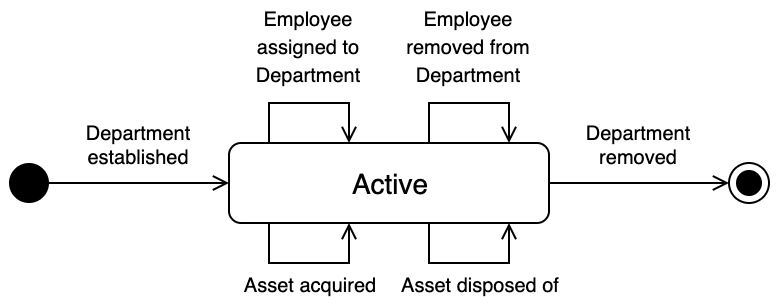
\includegraphics[width=0.8\textwidth]{figures/department_state_chart.png}
    \caption{Statechart diagram for Department}
    \label{fig:department_statechart}
\end{figure}
% After a department has been created, it stays active, until the department gets removed. During its active state, the department can have Employees added or removed, as well as assets Acquired or disposed of.
\newline

\Large  \textbf{Asset}  \normalsize
\par
\begin{figure}[H]
    \centering
    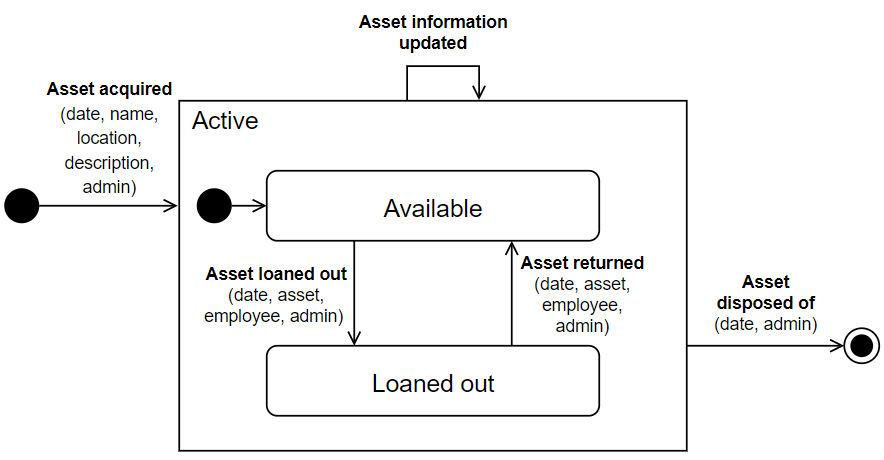
\includegraphics[width=0.8\textwidth]{figures/Asset_state_chart.png}
    \caption{Statechart diagram for Asset}
    \label{fig:asset_statechart}
\end{figure}



\Large  \textbf{Loan}  \normalsize
\par
\begin{figure}[H]
    \centering
    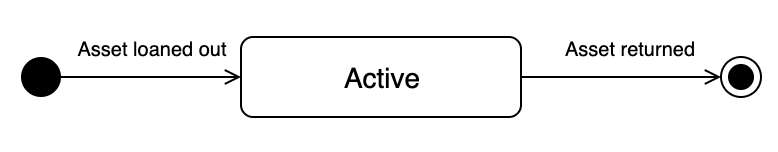
\includegraphics[width=0.8\textwidth]{figures/Loan_state_chart.png}
    \caption{Statechart diagram for Loan}
    \label{fig:loan_statechart}
\end{figure}

\Large  \textbf{Employee}  \normalsize
\par
\begin{figure}[H]
    \centering
    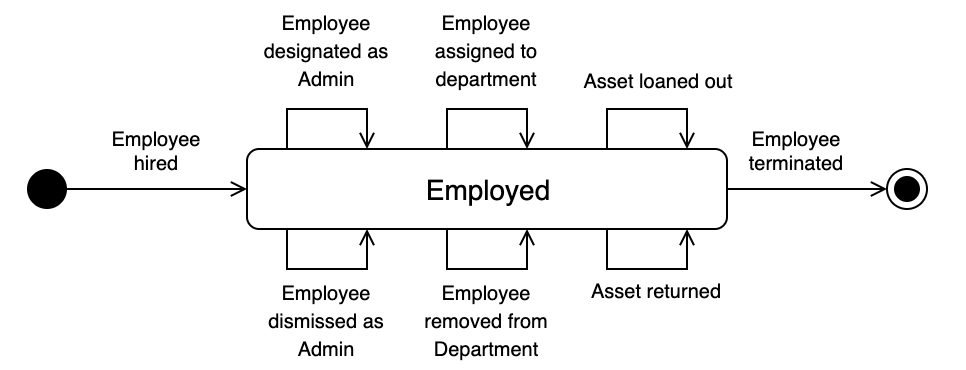
\includegraphics[width=1\textwidth]{figures/Employee_state_chart.png}
    \caption{Statechart diagram for Employee}
    \label{fig:employee_statechart}
\end{figure}

\Large  \textbf{Admin}  \normalsize
\par
\begin{figure}[H]
    \centering
    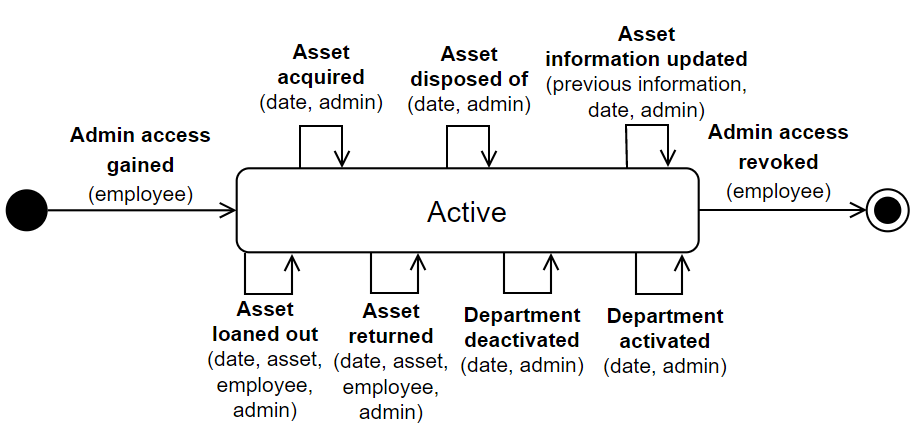
\includegraphics[width=0.8\textwidth]{figures/Admin_state_chart.png}
    \caption{Statechart diagram for Admin}
    \label{fig:admin_statechart}
\end{figure}

\todo[inline]{The following section needs to accommodate the admin in problem domain and not in the system (no mentions of tags and the other classes not present in the problem domain)}
% The admin class has a larger number of possible events, as this is a user with privileges to make changes in the system. An admin object is created when a user with administrator privileges logs in to the system. Then it is possible to add or remove objects, or edit those that are already present in the system. For example it is possible to add, remove, or edit tags on a particular asset, or comment on an asset. It is also possible for an admin to get a log of all the changes that has been made in the system. An administrator object is terminated when the user with administrator privileges logs off the system. This behavior is illustrated in figure \ref{fig:admin_statechart}.
\newline

With an understanding of how the different classes behave, the events has been added to an event table and further described in the next section.

